\documentclass[12pt]{article}
\usepackage{amssymb, amsmath, array}
\usepackage[xdvi]{graphics,color}
\usepackage[xdvi]{graphicx}
\usepackage{lscape}
\usepackage{pdflscape}
%\usepackage{xspace}
%\usepackage{enumerate}
\usepackage{threeparttable}
\usepackage{latexsym}

%\setlength{\textwidth}{18cm} \setlength{\textheight}{22.5cm}
%\setlength{\headheight}{-1cm} \setlength{\footskip}{1cm}
%\setlength{\oddsidemargin}{-1cm} \setlength{\evensidemargin}{0cm}
\setlength{\textwidth}{17.1cm} \setlength{\textheight}{22.5cm}
\setlength{\headheight}{-1cm} \setlength{\footskip}{1cm}
\setlength{\oddsidemargin}{-0.5cm}
\setlength{\evensidemargin}{-0.5cm}
\begin{document}
\baselineskip 20pt
\newtheorem{proposition}{Proposition}
\newtheorem{assumption}{Technical Assumption}

\begin{titlepage}
\title{{Labor Market Hours Constraints and Home Production}\thanks{We thank Daniel Aaronson, Charlie Brown, Karen Dynan, Dmitriy Stolyarov, and seminar and conference participants for helpful discussions and comments. Colin Motley, Hannah Farkas, and Ilaria Malisan provided superb research assistance. The views presented in this paper are those of the author and are not necessarily those of the Federal Reserve Board and its staff.}
\\ \vspace{0.5in}
}
  \author{Geng Li\thanks{Federal Reserve Board, Washington, DC 20551.  E-mail: Geng.Li@frb.gov. }  \\
          Federal Reserve Board
          \and Brett McCully\thanks{Collegio Carlo Alberto, Turin, Italy 10122.  E-mail: brett.mccully@carloalberto.org.} \\
          Collegio Carlo Alberto\vspace{.6in}}
\bigskip
\date{\today}
\maketitle\thispagestyle{empty}
\begin{abstract}
We document that labor market hours constraints are more pervasive than suggested by standard measures of labor market slack. We show that households adjust to such market hours constraints by increasing time spent on home production. 
\end{abstract}
\end{titlepage}
\clearpage

\section{Introduction}
A great deal of attention from policy makers and researchers has focused on the elevated level of workers who are part-time for economic reasons (PTER) since the Great Recession. While PTER is an important measure produced by the Bureau of Labor Statistics to measure labor market slack in the economy, we find that it significantly understates it. Using two nationally representative household surveys, we find that many full-time workers cannot work as many hours as they would prefer.

The survey data we use are the Panel Study of Income Dynamics (PSID) and the Health and Retirement Study (HRS).  Each survey asked respondents, “Would you have liked to work more if you could have found more work?” and, “Was there more work available on (any of your jobs) so that you could have worked more if you had wanted to?” We count a worker as facing work-hour constraints if he responded that he wanted to, but was not able to, work more hours. Separately, both surveys also collected data on how many hours an individual worked in a typical week, which let us identify the part-time workers and full-time workers.

We find that the share of part-time workers who were facing work-hour constraints match with the CPS PTER series very closely , indicating that the survey questions capture the PTER concepts well.  However, the share of all workers (part-time and full-time) who are work-hour constrained, while sharing a similar trend, is much higher than the CPS PTER rate, suggesting labor market slack is much more pervasive than the PTER rate alone implies.  Notably, the margin widened during the Great Recession and its aftermath (see figure below).  We then study the transition dynamics of such work-hour constraints and find that their persistence is quite high.  Fifty percent the constrained workers remain constrained the next year and, interestingly, the ratio is not sensitive to the duration of the experienced constraints.

We also explore the factors that drive workers into the constrained situations and how constrained workers deal with such scenarios.  We find that having an additional child in the family is not predictive for becoming constrained (holding earnings constant), while reductions in family income or increases in wage rates are associated with a greater likelihood of being work-hour constrained.  We also find that constrained workers increase home production, measured using housework hours and food-at-home share in total food expenses, to equalize the marginal utility of consumption and leisure in the constrained scenario.
\input{data.tex}
\section{Characterizing Working Hours Constraints}

\subsection{Occupations and Industries of the Constrained}
Working for what types of jobs and in which industries would make people more likely to have hours constraints?  Regarding occupations, as shown in table \ref{OCCIND}, the four occupations with highest odds of upside constraints include nonfarm laborers, operatives, transportation operators, and farm laborers, each with over or near 25 percent of workers being constrained.  The four occupations with lowest odds of upside constraints include sales, professionals, managers, and farmers.  The odds differences across occupations were larger. The average of the top four occupations was 28.6 percent, more than three times higher than the average of the bottom four occupations (8.9 percent).  Interestingly, the odds of upside and downside constraints were not inversely correlated across occupations.\footnote{The correlation coefficient is insignificant and small.}  For example, operatives ranked second for both constraints.

Turning to the odds of constraints in different industries, we find that the construction and entertainment industries had the highest odds of upside constraints (both above 25 percent), whereas the agriculture and finance industries have the lowest odds (near 10 percent).  Also, we note that the cross-industry dispersion of the upside-constraint odds is nearly 40 percent smaller than the cross-occupation dispersion.

\subsection{Trends of Working Hours Constraints}

The PSID estimates indicate that a large share of prime-age household heads were unable to work up to his/her desired number of hours in the labor market during the period from late 1960s to the middle of the 1980s. Among the constrained workers, over 60 percent can benefit financially and earn extra income should they be able to work more hours. Moreover, over 70 percent of the constrained worked full time. The significant prevalence of such labor hours constraints prompts the question whether the standard metrics such as share of people involuntarily working part time reveal the full picture of such frictions in the labor market and whether the survey-based measures of labor hours constraints may shed light on the state of the labor market over business cycles.

The most widely used indicator for tracking involuntary part-time workers is complied by the Bureau of Labor Statistics (BLS) using the Current Population Survey (CPS) data, which is often referred to as the share of working part-time for economic reasons (PTER). To introduce the PSID and the HRS data as useful additional data sources of studying labor market constraints, we show that the similarly defined series these two surveys share similar trends as the BLS PTER series.   Specifically, we show that the shares of involuntary part-time workers (those who were upside constrained and working fewer than 35 hours per week) measured in the PSID and HRS resemble the PTER rates estimated using the CPS data.  As shown in figure 1, during the overlapping sample period of 1967 to 1986, the CPS PTER series and the share of involuntary part-time workers in the PSID have similar levels and fluctuations, with the correlation of the two series being about 0.7, and about 0.6 for the detrended series. Both the PTER and the PSID series are highly countercyclical, with more people involuntarily working part-time or unable to work up to the ideal number of hours during recessions. Interestingly, peaks in the PSID series appear to overlap with NBER recession dates more closely than the PTER series.  Likewise, as shown in figure 2 the CPS PTER estimates of people older than 55 (a subpopulation comparable to the HRS sample) also share a trend similar to the share of upside constrained in the HRS, with both showing a substantial increase during the Great Recession.\footnote{The two series have a correlation coefficient of near 0.85 (0.74 for the detrended series).}  In addition, the CPS PTER estimates of the entire population (the black series) shared a similar trend as the estimates of those aged 55 and above.   All told, the PSID and HRS appear to have measured involuntary part-time work in a way consistent with the CPS PTER.

Because only a fraction of those upside constrained were part-time workers, the PTER series does not reveal the full extent to which the labor force was under working hours constraints. Indeed, as shown in figure 3, the overall prevalence of upside hour-constraints seen in both the PSID and HRS is much higher than the PTER rates, and such a gap is quite stable over the past several decades.  Second, despite the sizable gaps in their levels, the PSID and HRS work-hour-constraint estimates are highly correlated with the CPS PTER series over the respective overlapping period.

\subsection{Persistence of Working Hours Constraints}
To the best of our knowledge, most of the existing work pertinent to the transition dynamics of market work hours constraints uses the CPS data and focuses on involuntary part-time workers.  Because the CPS is a relatively short panel, the analysis is largely limited to the dynamics within a year.  As a result, relatively little is known regarding the reoccurrence and persistence of such constraints over a longer period, in particular among those who work full time. which can be an important element to further understanding of the nature and dynamics of these constraints. We present in table \ref{Markov} some simple statistics of the transition dynamics between years $t$ and $t+1$, and how the dynamics vary by part-time status. Because the upside constraints are much more prevalent and common than the downside constraints and have more direct welfare and monetary implications, our analysis will focus on such constraints.

Panel A shows the raw transition matrix of three states--upside constrained, unconstrained, and downside constrained--for all PSID household heads in our sample that can be linked between two years. We note that the upside constraints are rather persistent, with slightly fewer than half (48.2 percent) of the constrained workers remaining under such constraints one year later. Downside constraints, by contrast, are less persistent, with about one third of the constrained workers remaining so-constrained one year later. In addition, each year, 11.1 percent and 4.7 percent the unconstrained workers became upside and downside constrained, respectively.

Panel B illustrates how the transitions in and out of the upside constraints vary with the part-time status and presents four 2$\times$2 transition matrices that correspond to working full-time in both years, part-time in both years, changing from full-time to part-time, and from part-time to full-time, respectively.  The panel reveals several patterns: first, the upside constraints were fairly persistent across all four groups of workers, with the remaining constrained likelihood between 42 to 56 percent. Second, part-time workers appear to have a higher chance of remaining constrained, but those switch to working full-time in year $t+1$ had a better chance of escaping the constraints. Third, the unconstrained employees who changed from working full-time to working part-time had the highest chance of becoming constrained (17.7 percent), nearly twice as high as the odds of those who continued working full-time (9.8 percent). On balance, the statistics in panel B are consistent with the notion that many of those working part-time did so involuntarily and were vulnerable to such constraints.

Panel C takes a different perspective and presents the year $t+1$ status of those who were constrained in year $t$ by their part-time status in year $t$. Among the constrained full-time workers, about 85 percent stayed working full-time and 15 percent changed to working part-time. The full-time--part-time transition rate among the constrained appears to be higher than this rate for the entire labor force (see, for example, Borowczyk-Martins and Lal\'{e} 2019).\footnote{Another factor accounting for difference between our statistics and those reported in Borowczyk-Martins and Lal\'{e} (2019) is that the latter includes transitions into unemployment, other employment, and out of labor force, whereas our sample includes only those working positive hours in both year $t$ and year $t+1$.} Regardless whether changing to working part-time, roughly half of the workers remained constrained the next year. For part-time workers, about 55 percent of those constrained in year-$t$ worked full-time the next year.  Interestingly, 56 percent of those working full-time continued to report having working hours constraints, comparing with 42 percent of those remaining working part-time. The difference suggests that changing to working full-time was due to hours constraints. However, working full-time alone, for many workers, did not completely relax the constraints.

Finally, we note that the results presented in table \ref{Markov} are little changed when we restrict the sample to those who would receive additional pay if they worked extra hours.

\subsection{Factors Accounting for Transitions in and out of the Constraint}

We now estimate a econometric model to quantify the extent to which various demographic, labor market, and family income factors are associated with transition into and out of upside hours constraints.  We underscore that this is not a structural model that intends to uncover causal relationship.  Rather, we are interested in the degree to which such transitions can be accounted for by worker characteristics observed by econometricians. Specifically, we estimate the following logistic model for becoming upside constrained:

\begin{eqnarray}
Enter_{t, t+1}^i & = & \beta_0 + \beta_1 Age^i + \beta_2 Black^i + \beta_3 Edu^i + \beta_4 Lifecycle^i + \beta_5 \Delta Income_{t, t+1}^i \\
                 &   & + \beta_6 PT\sim FT_{t, t+1}^i + \beta_7 Year_t. \nonumber \label{logitbc} 
\end{eqnarray}

\noindent where $Enter_{t, t+1}^i$ is a indicator that is equal to one if worker $i$ became upside constrained in $t+1$, $Age$ is a third-order polynomial of worker's age, $Black$ a race dummy, and $Edu$ a vector of dummies indicating worker's educational attainment.  In addition $Lifecycle$ is a vector of lifecycle events including homeowner status, marital status, and number of children changes.  $\Delta Income$ includes log differences of family income and wage rate between $t$ and $t+$, and $PT-FT$ is a vector of full-time, part-time work status changes, with working full-time in both years being the omitted group.  Finally, we control for year fixed effects, $Year_t$.  The model is estimated using the sample of workers unconstrained in year $t$.  The estimated odds ratios are reported in column 1 of table \ref{TransitionReg}.  Odds ratios of continuous variables are evaluated for a one-standard deviation change.

Our results reveal that black workers on average are 72 percent more likely to become constrained than otherwise comparable white workers in a given year, and that the likelihood of becoming constrained substantially diminishes with education levels.  Regarding lifecycle events, workers remained married had a higher odds of becoming constrained relative to the workers remained single (the omitted group).  Moreover, having an additional child implies a 17 percent higher chance of becoming constrained, likely reflecting increased need of family spending. Indeed, a one-standard deviation increase in log of family income led to a nearly 45 percent reduction of the likelihood of being constrained, consistent with a positive income effect on labor supply.  Moreover, higher wage rates were associated with higher odds of becoming constrained, consistent with a positive substitution effect. Regarding part-time status changes, relatively to those who worked full-time in both years (the omitted group), other workers had a higher chance of becoming constrained, suggesting that such hours constraints were more likely to be binding for part-time workers.  Specifically, people who worked part-time in year $t+1$ had a 60 to 70 percent higher odds than the omitted group, and the year-$t$ part-time workers who became full-time in year $t+1$ has a 20 percent higher odds.  Moreover, we estimate the model using such unconstrained workers who would get extra pay for working extra hours (column 2). Most of the results are qualitatively the same as those in column (1), with the race estimates and the gradient of educational attainment estimates being somewhat smaller. One notable feature of the results presented is the low levels of the R-squared, 0.066 for the entire sample of year-$t$ unconstrained and 0.038 for the subsample of extra-pay eligible workers, which highlight that transitions into such constraints are only accounted for to a limited extent by observable factors.

We next study the transitions out of upside hours constraints, using a model similar to eq.(\ref{logitbc}). We add two additional variables, changed jobs and got additional jobs, to test if these were effective means of escaping such constraints.  We find that, among all workers reported being constrained in year $t$, black workers and workers with lower levels of education were less likely to escape the constraint (column 3).  Workers who remained married in both years also had a lower likelihood of escaping relative to those who stayed single. However, changes of number of children were not associated with the odds of becoming unconstrained. Consistent with a positive income effect and negative substitution effect on labor supply, higher family income and lower wages were associated with greater likelihood of no longer being constrained. In addition, workers working part-time in both years were less likely to become unconstrained than those working full-time in both years, though workers with full-time to part-time or part-time to full-time transitions appear to have similar odds as the omitted group.  Finally, our estimates suggest that constrained workers who changed job between year $t$ and $t+1$ had a greater odds of becoming unconstrained, but getting additional jobs did not change the likelihood.  The results estimated with the extra pay-eligible subsample (column 4) are largely the same, with the exception that race no longer predicts constraint status changes.  Similar to columns 1 and 2, the estimated values of R-squared were quite low.       
\section{Households Responses to Labor Hours Constraints}

\subsection{Conceptual Framework}

How do workers and their families deal with such labor hours constraints?  When worker want to work more hours than they are able to, the standard labor supply model implies that their marginal utility of leisure is not as large as the marginal utility associated with the additional income earned from working the marginal hour. To equalize these margins and achieve a second-best optimal, workers may increase home production or increase labor supply of other household members should it be available.\footnote{In addition to these two aspects, constrained workers may also reduce consumption, but saving, or increase borrowing.  We do not study these responses in this paper.} [I will add a stylized model that gives us increases in house work hours and spouse labor supply (for married households).  The model will be similar to the one in the earlier version but will consider spouse labor supply.  However, the model will not take into account intra-household bargaining.]

\subsection{Empirical Results}

\subsubsection{Single Households}

We first study how single workers respond to labor hours constraints. Specifically, we estimate the following model to test if single workers increase housework hours, $HWHead$, in response to upside labor hours constraints, $UC$, and reduce housework hours in response to downside constraints, $UC$.

\begin{equation} \label{housework}
HWHead = \alpha + \beta_u UC + \beta_d DC + \gamma Z + \theta Income + \phi Part-time + \tau Year,
\end{equation}

where demographic vector $Z$ includes an age polynomial and race and education dummies; $Income$ represents a vector of family income decile dummies, $Part-time$ indicates whether the head worked part-time in a given year; and the model also controls for year fixed effects.  We first estimate a similar linear regression, the results of which are reported in column 1 of table \ref{Single}. Our estimates indicate that single workers put, on average, about 47 more hours in housework during the year the worker was upside constrained---8.5\% higher than the unconstrained. However, housework hours did not appear to change when workers were under downside constraints. In addition, the estimated control variable coefficients suggest that households whose heads were black, had lower educational attainments, were single female, or were working part-time tend to have more housework hours.  Moreover, more children in the household tend to call for more housework. Note that the distribution of housework hours is non-normal and censored at zero.  Accordingly, we estimate a more robust specification, the tobit model.  The results, shown in column 2, are largely the same as in the linear model. The higher housework hours of constrained workers may reflect unobserved, persistent factors, such as household-specific preferences, instead of the labor hours constraints.  To quantify this potential effect, we estimate a longitudinal model, controlling for individual fixed effects.  The estimated increase of housework hours, 26 hours, is appreciably smaller than in the linear and tobit model, but remain sizeable and statistically significant. In addition to unobservable factors, the smaller estimated coefficient of $UC$ may also be attributable to the upside hours constraints being rather persistent. Finally, In all specification, downside hours constraints did not appear to have a significant bearing on housework hours.

We then reestimated these models using the subsample of workers who could earn extra money if working extra hours. Arguably, these were the workers with most tangible financial interests of working longer hours, therefore representing the most relevant hours constraints. The results, presented in columns 4-6, are qualitatively the same as the results estimated using the entire sample, with somewhat larger point estimates.  For example, the linear and tobit models show upside constrained workers had over 55 more housework hours.

\subsubsection{Married Households}
Turning to married households, these households had three ways to respond to heads' labor hours constraints as indicated by the model outlined above. Consider the upside constraints, first, the head could increase his own housework hours; second, the spouse could increase her housework hours; and third, the spouse could increase her market labor supply as she was not under such hours constraints. We test these channels in the framework of equation (\ref{housework}), replacing $HWHead$ with the three margins married households could adjust. In addition, we add spouse educational attainment as an additional control.  The results are presented in table \ref{Married}. 

The PSID define the male of a couple as the head of a married household. First, we note that married household heads' response to upside labor hours constraints (columns 1-2) were more muted than single male workers, and this pattern held in both the tobit (31 versus 47 hours) and longitudinal regressions (10 versus 26 hours). In addition, like single workers, housework hours of married households did not appear to change for downside constraints ($DC$). Turning to wife's housework, as shown in columns 3-4, heads' being unable to work more hours appeared to be associated with lower wife's time input for home production, as the coefficient of $UC$ is negative in both specifications. In contrast, wives of heads with downside hours constraints had more hours of housework than otherwise comparable spouses. There could be two factors accounting for why heads' labor hours constraints did not lead to the same change to wives' housework hours as they did on their own housework hours.  First, wives had a large number of housework hours, around 1,400 hours per year, regardless heads' labor hours constraint status, comparing with about heads' 300 housework hours.  Therefore, the marginal cost of wives' housework could be so high that increasing it even when heads were constrained was not desirable.  Second, if wives chose to increase market labor supply in response to heads' labor hours constraints, that will reduce their available time for housework.

Columns 5-9 explore wives' market labor supply changes, on both the extensive and intensive margins. We first replace the dependent variable of equation (\ref{housework}) with a dummy of whether wife worked in a given year and estimate a logistic model. The estimated odds ratios indicate that wives of upside constrained heads were over 20 \% more likely to work in that year. However, as in many of the previous results, downside constraints did not have a significant bearing on wife work status. In addition, our estimates reveal that wives' propensity of working declined with heads' education and rose with own education. The former likely reflects an income effect of wife labor supply, whereas the latter reveals a substitution effect as more educated women earn higher wages. Also, we note that female labor force participation rate in the earlier part of our PSID sample period remained low. We next study if wives who were not working before would start working when heads were constrained, by estimating the previous model using a subsample of wives not working in year $t-1$.  As shown in column 6, relative to other comparable spouses, wives are more 16 percent likely to enter the labor market during the year when their husbands were not able to work more hours as desired.

On the intensive margin, we find that working wives whose spouses were upside constrained tended to work more hours.  First, as shown in column 7, upside constrained heads' working wives were 8 percent less likely to work part-time, whereas the downside constrained heads' spouses were 20 percent more likely to do so.  Finally, the cross-sectional and longitudinal analysis indicate that wives' working hours are estimated to be 53 and 36 hours longer, respectively, in the year their husbands are upside constrained. The downside constraints were not strongly associated with wives working hours.

To summarize, we find that single workers appeared to increase housework hours significantly when they were not able to work as many hours as desired in the labor market.  For married households, the adjustments on housework were more muted. In contrast, wives tended to increase their market labor supply under such constraints, either by entering the labor force or by working longer hours. Results presented in table \ref{Married} are estimated using the entire sample of married households. Reestimating the models using the subsample of extra-pay eligible workers yields qualitatively the same results.

\subsection{Food-out Ratios}
The PSID analysis, while comprehensive, draws on a sample the last observation of which was collected almost 35 years ago.  We supplement the study with an analysis of the HRS data, which cover the recent year. First, we note that unlike in the PSID sample, we did not find labor supply variations of HRS wives associated with their husbands' hours constraints. The difference likely reflects the sample age differentials.  The youngest household heads in the HRS were 50 years old, and wives' labor supply flexibility is more limited at that age.  Indeed, when we repeat the analysis using the PSID subsample of households aged 50 years and older, we no longer see spouse labor supply changes.
 
We therefore focus on the potential effect of labor hours constraints on housework and home production.  As discussed earlier, the HRS data collect housework hours data but in a year different from labor hours constraints data. As a result, we use food-out ratio, defined as the share of eating expenditures in total food expenditures as a proxy of housework, with lower food-out ratio indicating greater home production. This ratio can be constructed in both the PSID and HRS data, contemporaneous to the labor hours constraints data. Another difference between the two surveys is that the food-out ratios differed by a large margin between single and married households in the PSID data but were close in the HRS data, which is also mainly due to age differences of the two survey. Food-out ratios were similar in the PSID subsample of households older than 50.

We first confirm if the housework hour variations we find in the PSID manifest in food-out ratios. Doing so will further validate using the food-out ratio as a proxy of housework. As shown in column 1-4 of table \ref{HRS}, estimating a tobit specification of equation (\ref{housework}) reveals that, for single and married households, upside hours constraints were associated with food-out ratios 1.5 and 0.9 percentage point (about 6 percent of mean ratio) lower, respectively.  The estimated reduction are greater for extra-pay eligible workers at around 2 percentage points.

Turning to the HRS sample, which we estimate the model pooling single and married households together, constrained households were estimated to have a 2 percentage points lower food-out ratio, or 8 percent of the mean ratio of unconstrained households. Interestingly, the estimate is appreciably smaller among extra-pay eligible households but remains statistically significant.\footnote{The difference relative to the PSID in part reflects variations in how extra-pay eligibility information was collected in both surveys as the labor market evolved over the past several decades.}

\input{conclusion.tex}
******Cite Baker and Yannelis
\clearpage

\begin{figure}[h]
\begin{center}
\caption{Trends of Constrained Workers over Fifty Years \label{inf}}
\includegraphics[width=5in, height=4in]{figure1.eps}
\end{center}
\end{figure}

\newpage

\begin{center}
\footnotesize
\begin{threeparttable}
\caption{Variables Definition and Years Available} \label{Variable}
\label{Variable}
\begin{tabular}{llll}

\hline\hline \\
Definition                                     &PSID                     &     &HRS                     \\
\hline\hline \\
Head Upside Constrained --- Wanted to work     &1967 - 1986              &     &All waves               \\
more hours but were not able to (UC)           &                         &     &                        \\ \\
Head Downside Constrained --- Wanted to        &1967 - 1986              &     &All waves               \\
work fewer hours but were not able to (DC)     &                         &     &                        \\ \\
%Wife Upside Constrained --- Same as head       &1970 - 1975              &     &All waves               \\ \\
Ideal number of market hours                   &NA                       &     &All waves               \\ \\
Hours spent on housework                       &1968 - 1986              &     &NA (off year only)      \\
by head and wife (HWHead, HWWife)              &                         &     &                        \\ \\
Ratio between food consumed out and            &1969 - 1986 except 1973  &     &All waves except 1998   \\
total food expenditure (Food-out ratio)        &                         &     &                        \\ \\
%Number of vacation weeks taken (Weeks)         &1967 - 1986              &     &NA                      \\
\hline\hline \\[-1ex]
\end{tabular}
\begin{tablenotes}
\item[] \footnotesize{The PSID data availabilities refer to the
waves of 1968 -- 1986.  The HRS data have eight waves, every other
year from 1992 to 2006.}
\end{tablenotes}
\label{var}
\end{threeparttable}
\end{center}


\begin{center}
\footnotesize
\begin{threeparttable}
\caption{Summary Statistics} \label{Summary}
\begin{tabular}{lcccccc}
\hline \hline \\[-1ex]
                            &\multicolumn{2}{c}{\underline{Upside Constrained}}
                            &\multicolumn{2}{c}{\underline{Downside Constrained}}
                            &\multicolumn{2}{c}{\underline{Not Constrained}}                      \\[.5em]
                                            &PSID   &HRS      &PSID   &HRS      &PSID   &HRS      \\
                                            & (1)   & (2)     &(3)    & (4)     & (5)   &(6)      \\
\hline \\
\% household $\times$ year                  &18.7   &11.4     &5.7    &8.2      &75.6   &80.5     \\ \\
\% households ever constrained              &52.3   &23.3     &24.8   &17.1     &35.8   &62.5     \\ \\
By how many hours                           &NA     &451      &NA     &731      &NA     &NA       \\
                                            &       &(323)    &       &(440)    &       &         \\
Demographic Characteristics &&&&&& \\
\hspace{.3in} Age                           &37.6   &56.3     &41.3   &57.1     &40.9   &57.6     \\
                                            &(11.2) &(4.5)    &(12.0) &(4.3)    &(12.1) &(4.9)    \\[1ex]
\hspace{.3in} White (\%)                    &80.2   &81.5     &88.9   &86.9     &88.9   &87.0     \\[1ex]
\hspace{.3in} Below high school (\%)        &34.3   &13.6     &23.0   &9.0      &22.6   &11.4     \\[1ex]
\hspace{.3in} High school graduate (\%)     &38.6   &30.6     &36.3   &32.5     &33.3   &27.3     \\[1ex]
\hspace{.3in} Some college and college (\%) &27.1   &55.9     &40.7   &58.3     &44.1   &61.3     \\[1ex]
\hspace{.3in} Married (\%)                  &73.7   &61.7     &72.9   &65.6     &73.8   &68.9     \\ \\

Income (1986 dollars)and hours worked       &       &         &       &         &       &         \\
\hspace{.3in} Family income(\$thousands)    &29.3   &35.9     &40.5   &47.8     &39.5   &52.8     \\
                                            &(17.3) &(31.9)   &(24.3) &(45.9)   &(25.7) &(61.7)   \\[1ex]
\hspace{.3in} Hours worked                  &1,968  &2,022    &2,301  &2,299    &2,180  &2,144    \\
                                            &(525)  &(487)    &(566)  &(479)    &(610)  &(559)    \\
\hspace{.3in} Working part time             &28.2   & 22.3    &12.9   & 8.2     &19.2   & 25.2    \\ \\

Home production                             &       &         &       &         &       &         \\
\hspace{.3in} Unmarried head housework hours&629    &NA       &539    &NA       &559    &NA       \\
                                            &(471)  &         &(425)  &         &(443)  &         \\[1ex]
\hspace{.3in} Married head housework hours  &326    &NA       &292    &NA       &291    &NA       \\
                                            &(383)  &         &(342)  &         &(342)  &         \\[1ex]
\hspace{.3in} Married wife housework hours  &1,385  &NA       &1,469  &NA       &1,420  &NA       \\
                                            &(799)  &         &(781)  &         &(781)  &         \\[1ex]
\hspace{.3in} Unmarried food-out ratio (\%) &25.5   &18.3     &31.5   &22.8     &31.2   &22.0     \\[1ex]
\hspace{.3in} Married food-out ratio (\%)   &14.3   &18.8     &18.1   &22.9     &17.8   &22.1     \\[1ex]
%\hspace{.3in} Wife housework hours          &1,490  &NA       &1,490  &NA       &1,460  &NA       \\
%                                            &(843)  &         &(833)  &         &(829)  &         \\[1ex]
\hline\hline \\[-1ex]
\end{tabular}
\begin{tablenotes}
\item[] \footnotesize{All statistics are computed using the PSID
and HRS weights. Standard deviations of continuous variables are
reported in parenthesis.}
\end{tablenotes}
\label{sum}
\end{threeparttable}
\end{center}

\clearpage

\begin{center}
\scriptsize
\begin{threeparttable}
\caption{Occupation and Industry} \label{OCCIND}
\begin{tabular}{lcclcclcclc}
\hline \hline \\[-1ex]
                            \multicolumn{5}{c}{Occupation} &&\multicolumn{5}{c}{Industry} \\
                            (1) & (2) && (3) & (4) \\[.5em]
\hline\\[-1ex]
                            \multicolumn{2}{c}{\underline{Upside}}&&\multicolumn{2}{c}{\underline{Downside}}&&\multicolumn{2}{c}{\underline{Upside}}&&\multicolumn{2}{c}{\underline{Downside}} \\
                            Laborers				  		& 32.5	&&	Farm laborers	    &	6.9         && Construction	        & 29.3    &&    Mining	             & 7.7 \\[1ex]
                            Operatives						& 30.0  &&  Operatives	        &	6.3         && Entertainment     	& 26.0    &&    Manufacturing	     & 6.7 \\[1ex]
                            Trans. operators   		        & 27.1  &&  Craftsman	        &	6.2         && Personal Services    & 23.3    &&    Public Admin	     & 6.3 \\[1ex]
                            Farm laborers					& 24.7  &&  Trans. operators    &	6.0         && Manufacturing	    & 20.7    &&    Trans., Comm., Util. & 6.2 \\[1ex]
                            Service workers				    & 23.4  &&  Manager	            &	6.0         && Trans., Comm., Util.	& 20.0    &&    Wholesale and Retail & 5.7 \\[1ex]
                            Craftsman						& 23.0  &&  Professional	    &	6.0         && Business and Repair  & 18.2    &&    Business and Repair	 & 5.3 \\[1ex]
                            Clerical						& 21.3  &&  Clerical      	    &	5.4         && Mining	            & 16.7    &&    Agriculture	         & 4.7 \\[1ex]
                            Priv. hhld. workers  	        & 19.1  &&  Service workers	    &	5.4         && Public Admin.       	& 16.3    &&    Construction	     & 4.6 \\[1ex]
                            Sales							& 11.6  &&  Farmers	            &	3.2         && Wholesale and Retail	& 16.1    &&    Professional	     & 4.5 \\[1ex]
                            Professional					& 11.2  &&  Sales	            &	3.2         && Professional	        & 13.5    &&    Personal Services	 & 4.5 \\[1ex]
                            Manager							& 7.5   &&  Laborers	        &	3.0         && Agriculture	        & 11.6    &&    Finance	             & 4.2 \\[1ex]
                            Farmers							& 5.3   &&  Priv. hhld workers  &	1.5         && Finance              & 10.2    &&    Entertainment	     & 2.3 \\
\hline\hline \\[-1ex]
\end{tabular}
\begin{tablenotes}
\item[] All statistics are computed using the PSID weights.
\end{tablenotes}
\label{sum}
\end{threeparttable}
\end{center}

\begin{center}
\footnotesize
\begin{threeparttable}
\caption{Transition Matrix of Constraint Status} \label{Markov}
\begin{tabular}{lccc}
\hline \hline \\[-1ex]
\multicolumn{4}{c}{Panel A Overall Transition Matrix (\%)} \\
\hline \\[-1ex]
                          & \multicolumn{3}{c}{Year t+1}  \\
Year t                    & Upside constrained &  Unconstrained & Downside constrained \\ \\
Upside constrained        &  48.2              &  49.2          & 2.6                  \\ \\
Unconstrained             &  11.1              &  84.2          & 4.7                  \\ \\
Downside constrained      &  7.6               &  62.3          & 30.1                 \\
\hline \\[-1ex]
\end{tabular}

\begin{tabular}{lccccc}
\multicolumn{6}{c}{Panel B Upside Constraint Transitions by Part-Time Status (\%)} \\
\hline \\[-1ex]
                          & \multicolumn{2}{c}{Full-time only}  && \multicolumn{2}{c}{Part-time only}\\
\cline{2-3} \cline{5-6}

                          & Constrained &  Unconstrained && Constrained & Unconstrained \\ \\
Constrained               &  52.9       &  47.2          && 55.9        & 44.1          \\ \\
Unconstrained             &  9.8        &  90.2          && 12.9        & 87.1          \\ \\

                          & \multicolumn{2}{c}{Full-time to part-time}  && \multicolumn{2}{c}{Part-time to full-time}\\
\cline{2-3} \cline{5-6}

                          & Constrained &  Unconstrained && Constrained & Unconstrained \\ \\
Constrained               &  49.3       &  50.7          && 42.4        & 57.6          \\ \\
Unconstrained             &  17.7       &  82.3          && 11.5        & 88.5          \\ \\
\hline
\end{tabular}

\begin{tabular}{lccccc}
\multicolumn{6}{c}{Panel C Subsequent-Year Status of the Upside Constrained (\%)} \\
\hline \\[-1ex]
                          & \multicolumn{5}{c}{Year t+1}\\
\cline{2-6}

                          & \multicolumn{2}{c}{Full-time} && \multicolumn{2}{c}{Part-time}  \\
Year t                    & Constrained &  Unconstrained  && Constrained & Unconstrained \\ \\
Full-time                 & 40.3        &  45.2           && 7.1         & 7.3          \\ \\
Part-time                 & 31.5        &  24.8           && 18.5        & 25.2          \\ \\
\hline
\end{tabular}
\begin{tablenotes}
\item[] \footnotesize{All statistics are computed using the PSID weights.}
\end{tablenotes}
\label{sum}
\end{threeparttable}
\end{center}

\clearpage

\begin{center}
\footnotesize
\begin{threeparttable}
\caption{Factors Associated with Transitions into and out of Constraints} \label{TransitionReg}
\begin{tabular}{lccccc}
\hline \hline \\[-1ex]
                          &\multicolumn{2}{c}{Became upside constrained} && \multicolumn{2}{c}{Escaped upside constraints}\\
                          & (1)           & (2)           &&      (3)      & (4)           \\
Head characteristics      &&&&&\\[1ex]
\hspace{.1in}Black                     &       1.724***&       1.399***&&       0.899** &       1.000   \\
                                       &     (0.071)   &     (0.069)   &&     (0.040)   &     (0.053)   \\
\hspace{.1in}High school               &       0.671***&       0.713***&&       1.121** &       1.091   \\
                                       &     (0.031)   &     (0.039)   &&     (0.058)   &     (0.066)   \\
\hspace{.1in}Some college              &       0.497***&       0.594***&&       1.385***&       1.273***\\
                                       &     (0.030)   &     (0.044)   &&     (0.096)   &     (0.103)   \\
\hspace{.1in}College                   &       0.262***&       0.446***&&       1.791***&       1.468***\\
                                       &     (0.019)   &     (0.050)   &&     (0.172)   &     (0.186)   \\
Lifecycle events                       &               &               &&               &               \\[1ex]
\hspace{.1in}Became homeowner          &       1.090   &       1.120   &&       0.983   &       0.955   \\
                                       &     (0.073)   &     (0.095)   &&     (0.081)   &     (0.092)   \\
\hspace{.1in}Got married               &       0.909   &       0.787   &&       1.019   &       0.994   \\
                                       &     (0.116)   &     (0.129)   &&     (0.147)   &     (0.165)   \\
\hspace{.1in}Remain married            &       1.185***&       1.246***&&       0.868***&       0.895*  \\
                                       &     (0.053)   &     (0.068)   &&     (0.043)   &     (0.054)   \\
\hspace{.1in}Divorced/Separated        &       1.004   &       0.985   &&       1.196   &       1.317   \\
                                       &     (0.122)   &     (0.152)   &&     (0.179)   &     (0.231)   \\
\hspace{.1in}Change number of children &       1.174***&       1.263***&&       0.954   &       1.039   \\
                                       &     (0.062)   &     (0.082)   &&     (0.057)   &     (0.074)   \\
Income and employment                  &               &               &&&\\[1ex]
\hspace{.1in}Change log(faminc)        &       0.559***&       0.575***&&       1.394***&       1.429***\\
                                       &     (0.032)   &     (0.046)   &&     (0.093)   &     (0.122)   \\
\hspace{.1in}Change log(wage)          &       1.191***&       1.251***&&       0.860** &       0.895   \\
                                       &     (0.063)   &     (0.092)   &&     (0.052)   &     (0.073)   \\
\hspace{.1in}F.T. to P.T.              &       1.695***&       1.503***&&       1.042   &       1.067   \\
                                       &     (0.082)   &     (0.091)   &&     (0.063)   &     (0.077)   \\
\hspace{.1in}P.T. to F.T.              &       1.221***&       1.109   &&       1.100   &       1.096   \\
                                       &     (0.076)   &     (0.086)   &&     (0.064)   &     (0.077)   \\
\hspace{.1in}P.T. to P.T.              &       1.606***&       1.472***&&       0.714***&       0.753*** \\
                                       &     (0.091)   &     (0.110)   &&     (0.041)   &     (0.054)    \\
\hspace{.1in}Changed jobs              &               &               &&       1.237***&       1.251*** \\
                                       &               &               &&     (0.058)   &     (0.071)    \\
\hspace{.1in}Got additional job        &               &               &&       1.045   &       1.092    \\
                                       &               &               &&     (0.066)   &     (0.084)    \\
Controlled for                         &               &               &&               &               \\[1ex]
\hspace{.1in} Head age polynomial      & Yes           & Yes           &&  Yes          &  Yes          \\
\hspace{.1in} Year fixed effects       & Yes           & Yes           &&  Yes          &  Yes          \\[1ex]
Pseudo R-squared                       & 0.066         & 0.038         &&  0.020        &  0.014        \\
N                                      &       41,353  &       20,114  &&      13,671   &       9,247   \\ \hline
\end{tabular}
\begin{tablenotes}
\item[] \footnotesize{}
\end{tablenotes}
\label{sum}
\end{threeparttable}
\end{center}

\clearpage

\begin{center}
\begin{threeparttable}
\caption{Effects of Market Work Hours Constraints on Singles' Housework Hours} \label{Single}
\begin{footnotesize}
\begin{tabular}{lccccccc}
\hline \hline
                     & \multicolumn{3}{c}{Whole sample}  && \multicolumn{3}{c}{Can get extra pay} \\
\cline{2-4} \cline{6-8} \\
                     &OLS            &Tobit          &Panel          &&OLS            &Tobit          &Panel           \\
                     &(1)            &(2)            &(3)            &&(5)            &(6)            &(7)             \\
\hline \\
Upside Constrained   &        46.5***&        47.6***&        26.3***&&        56.1***&        57.5***&        29.1**  \\
                     &      (11.7)   &      (10.1)   &      (10.0)   &&      (14.1)   &      (12.9)   &      (14.1)    \\
Downside Constrained &        -3.6   &        -5.8   &       -13.1   &&       -13.9   &       -18.8   &        -5.4    \\
                     &      (19.1)   &      (18.4)   &      (17.6)   &&      (23.3)   &      (23.7)   &      (24.2)    \\
Black                &        34.5** &        36.2***&               &&        36.0** &        38.6***&                \\
                     &      (15.2)   &       (9.4)   &               &&      (17.6)   &      (12.1)   &                \\
High school          &       -21.1   &       -16.6   &               &&        -7.6   &        -0.2   &                \\
                     &      (17.6)   &      (11.1)   &               &&      (20.4)   &      (14.3)   &                \\
Some college         &       -59.3***&       -52.5***&               &&       -46.6** &       -37.4** &                \\
                     &      (20.4)   &      (13.4)   &               &&      (22.7)   &      (17.3)   &                \\
College              &      -114.2***&      -106.3***&               &&       -76.5** &       -64.2***&                \\
                     &      (23.0)   &      (14.7)   &               &&      (30.3)   &      (24.0)   &                \\
Number of children   &        86.7***&        85.9***&        39.9***&&        89.9***&        89.0***&        39.2*** \\
                     &       (9.0)   &       (4.1)   &       (6.2)   &&      (10.1)   &       (5.6)   &       (8.9)    \\
Number of adults     &       -14.0   &       -22.8***&        -4.0   &&       -12.2   &       -19.0** &         5.8    \\
                     &      (10.7)   &       (6.5)   &       (8.5)   &&      (13.7)   &       (9.1)   &      (13.1)    \\
Single female        &       236.8***&       269.7***&               &&       223.6***&       253.8***&                \\
                     &      (14.6)   &       (9.6)   &               &&      (18.5)   &      (13.1)   &                \\
Working part-time    &        57.2***&        61.1***&        24.9** &&        47.6***&        49.9***&        15.6    \\
                     &      (11.7)   &       (9.2)   &       (9.7)   &&      (14.9)   &      (12.6)   &      (14.1)    \\
N                    &       13,451  &       13451   &       13,451  &&        7,038  &        7,038  &        7,038   \\

\hline\hline
\end{tabular}
\end{footnotesize}
\begin{tablenotes}
\item[] \footnotesize{\noindent 90\% 95\% and 99\% statistical
significance are denoted by *, ** and ***, respectively.}
\end{tablenotes}
\label{Analysis}
\end{threeparttable}
\end{center}

\clearpage
\begin{landscape}
\begin{center}
\begin{threeparttable}
\caption{Effects of Market Work Hours Constraints on Married Households} \label{Married}
\begin{footnotesize}
\begin{tabular}{lcccccccccccc}
\hline \hline
                     & \multicolumn{5}{c}{Housework hours}  && \multicolumn{6}{c}{Wife work status} \\
\cline{2-6} \cline{8-13} \\
                     & \multicolumn{2}{c}{\underline{Head}} && \multicolumn{2}{c}{\underline{Wife}}  && \multicolumn{2}{c}{\underline{Extensive margin}} && \multicolumn{3}{c}{\underline{intensive margin}} \\
                     &               &               &&               &               && Work          & Start to work && Work part-time& Work hours    & Work hours \\
                     &Tobit          &Panel FE       && Tobit         & Panel FE      && Logistic      & Logistic      && Logistic      & OLS           & Panel FE      \\
                     &(1)            &(2)            &&(3)            &(4)            &&(5)            &(6)            && (7)           & (8)           & (9)   \\
\hline \\[-1ex]
Upside Constrained   &       30.68***&       10.41** &&       -24.7** &       -16.4   &&       1.22***&        1.16** &&        0.92*  &       53.48***&       36.52***\\
                     &      (6.79)   &      (5.30)   &&      (10.7)   &      (10.7)   &&     (0.05)   &      (0.07)   &&      (0.04)   &     (15.50)   &     (11.52)   \\
Down Constrained     &      -11.48   &       -9.28   &&        35.1*  &        14.6   &&       0.96   &        1.11   &&        1.21***&      -15.77   &      -16.21   \\
                     &     (12.31)   &      (9.12)   &&      (19.3)   &      (18.4)   &&     (0.06)   &      (0.13)   &&      (0.09)   &     (27.40)   &     (19.94)   \\
Black                &       68.26***&               &&      -310.5***&               &&       1.72***&        1.26***&&        0.56***&      262.99***&               \\
                     &      (6.76)   &               &&      (10.6)   &               &&     (0.10)   &      (0.09)   &&      (0.03)   &     (20.51)   &               \\
Head Education       &               &               &&           .   &               &&              &               &&               &               &               \\
\;\;\;High school    &       57.40***&               &&        68.2***&               &&       0.81***&        0.90   &&        1.47***&     -114.63***&               \\
                     &      (7.71)   &               &&      (11.9)   &               &&     (0.05)   &      (0.07)   &&      (0.10)   &     (25.56)   &               \\
\;\;\;Some college   &      102.37***&               &&        41.7***&               &&       0.79***&        0.95   &&        1.64***&     -180.12***&               \\
                     &      (9.41)   &               &&      (14.8)   &               &&     (0.06)   &      (0.09)   &&      (0.14)   &     (30.31)   &               \\
\;\;\;College        &      102.79***&               &&        56.8***&               &&       0.59***&        0.87   &&        2.52***&     -324.47***&               \\
                     &     (10.37)   &               &&      (16.4)   &               &&     (0.05)   &      (0.09)   &&      (0.24)   &     (34.27)   &               \\
Wife Education       &               &               &&           .   &               &&              &               &&               &               &               \\
\;\;\;High school    &       35.05***&               &&        16.1   &               &&       1.07   &        1.01   &&        0.96   &       -0.92   &               \\
                     &      (8.85)   &               &&      (13.5)   &               &&     (0.07)   &      (0.09)   &&      (0.07)   &     (28.70)   &               \\
\;\;\;Some college   &       75.37***&               &&       -67.2***&               &&       1.43***&        1.41***&&        0.94   &       -1.82   &               \\
                     &      (9.31)   &               &&      (14.4)   &               &&     (0.10)   &      (0.13)   &&      (0.07)   &     (28.62)   &               \\
\;\;\;College        &       71.86***&               &&      -146.5***&               &&       2.07***&        1.39** &&        1.60***&      -73.87** &               \\
                     &     (12.33)   &               &&      (19.5)   &               &&     (0.21)   &      (0.19)   &&      (0.16)   &     (36.17)   &               \\
Num. children        &       -5.68** &       -3.14   &&       150.4***&       122.8***&&       0.83***&        0.91***&&        1.23***&      -70.96***&      -57.06***\\
                     &      (2.24)   &      (2.19)   &&       (3.4)   &       (4.4)   &&     (0.01)   &      (0.02)   &&      (0.02)   &      (7.27)   &      (5.11)   \\
Num. adults          &      -35.52***&       -6.67   &&        62.6***&        57.0***&&       0.87***&        0.88***&&        1.13***&      -71.88***&     -101.09***\\
                     &      (4.96)   &      (4.30)   &&       (7.5)   &       (8.7)   &&     (0.03)   &      (0.04)   &&      (0.05)   &     (16.49)   &      (9.51)   \\
Work part time       &       45.98***&       13.76** &&      -112.7***&       -55.4***&&       1.32***&        1.12   &&        0.92*  &       80.45***&       56.89***\\
                     &      (7.75)   &      (6.24)   &&      (12.2)   &      (12.6)   &&     (0.06)   &      (0.08)   &&      (0.05)   &     (17.67)   &     (13.66)   \\
N                    &       30,743  &       30,743  &&       30,743  &       30,743  &&      38,337  &       11,031  &&       24,960  &       20,740  &       22,141  \\\hline\hline
\end{tabular}
\end{footnotesize}
\end{threeparttable}
\end{center}
\end{landscape}

\newpage
\begin{center}
\begin{threeparttable}
\caption{Market Hours Constraints and Food-Out Shares } \label{HRS}
\begin{footnotesize}
\begin{tabular}{lccccccccc}
\hline \hline
Sample            &\multicolumn{5}{c}{PSID}           &&\multicolumn{2}{c}{HRS}  \\[1ex]
\cline{2-6}\cline{8-9}
                     & \multicolumn{2}{c}{Whole sample}  && \multicolumn{2}{c}{Can get extra pay} && Whole sample & Can get extra pay \\
\hline \\[-1ex]
                     &Unmarried          & Married       &&Unmarried        & Married             &&              &         \\
                     &(1)                &(2)            &&(3)              &(4)                  &&(5)           &(6)            \\
\hline \\
$\beta_u$            &      -1.474** &      -0.856***&&      -1.737** &      -2.063***&&      -2.034***&      -0.771***\\
                     &     (0.689)   &     (0.193)   &&     (0.807)   &     (0.452)   &&     (0.534)   &     (0.235)   \\
$\beta_d$            &       0.714   &       0.053   &&       2.809** &       0.123   &&       0.147   &       0.066   \\
                     &     (1.090)   &     (0.356)   &&     (1.367)   &     (0.505)   &&     (0.627)   &     (0.479)   \\
N                    &       14,823  &       33,843  &&        8,095  &       32,787  &&       24,617  &       18,614  \\
\hline\hline
\end{tabular}
\end{footnotesize}
\begin{tablenotes}
\item[] \footnotesize{\noindent 90\% 95\% and 99\% statistical
significance are denoted by *, ** and ***, respectively.}
\end{tablenotes}
\end{threeparttable}
\end{center}















\end{document}

